\documentclass{article}
\usepackage{geometry}
\geometry{a4paper, scale=0.8}

\usepackage[utf8]{inputenc}
\usepackage{ctex}
\usepackage{assignpkg}
\usepackage{amsmath}
\usepackage{amssymb}
\usepackage[colorlinks, linkcolor=red]{hyperref}

\studentIds{202XX80XXXXXXXX}{}
\studentNames{XXX}{}

\assignmentNumber{}

\date{\today}

\begin{document}

\makecover
\section*{椭圆曲线加法结合律的证明}
说明:
\begin{itemize}
\item[1]
以下讨论中所有的点与直线均是在射影平面下的点和直线。仿射平面内无交点的两条平行线在射影平面内将有交点$O$,为无穷远点。
\item[2]
参考资料为\href{https://math.mit.edu/classes/18.783/2019/LectureNotes2.pdf}{lecture notes 2}。
\end{itemize}

设$P,Q,R$ 为域 $K$ 上的椭圆曲线 $E$  上的任意三个点, $O$ 为单位元,即无穷远点。由椭圆曲线加法的定义,我们知道和为 $O$ 的两个与无穷远点$O$在同一直线上,设
\begin{itemize}
\item[]
$P,R,-(P+R)$ 位于直线 $m_0$ 上。\\
$P,Q,-(P+Q)$ 位于直线 $l_0$ 上。\\
$-(P+Q),P+Q,O$ 在直线 $m_2$ 上。\\
$-(P+R),P+R,O$ 在直线 $l_2$ 上。\\
$R+P,Q,T=-((R+P)+Q)$ 在直线 $m_1$ 上。\\
$R,P+Q,S=-(R+(P+Q))$ 在直线 $l_1$ 上。\\
\end{itemize}
将这些点的与直线的关系画出来,则如下图1所示。\\
\begin{figure}[htbp]
\centering
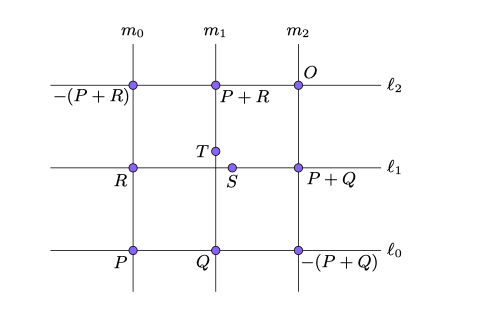
\includegraphics[scale=0.8]{elliptical.png}
\caption{图源:\href{https://math.mit.edu/classes/18.783/2019/LectureNotes2.pdf}{lecture notes 2}(点击红字可访问网址)}
\end{figure}
要证明加法满足结合律$(R+P)+Q=R+(P+Q)$,证明 $S=T$ 即可。\\

采用反证法。假设一般情况下 $S= T$ 不成立,即 $S\ne T$ 。

令$ g(x,y,z) $为直线 $l_0(x,y,z)=0,l_1(x,y,z)=0,l_2(x,y,z)=0$ 的齐次坐标方程的乘积,记 $g(x,y,z)=l_0(x,y,z)l_1(x,y,z)l_2(x,y,z)=l_1l_2l_3$ 。同理,令 $h(x,y,z)=m_0m_1m_2$ ,则 $g,h$ 都为三次齐次多项式。

由于 $T$ 不在$l_1,l_2,l_3$上,故$l_1(T)\ne 0 ,l_2(T)\ne 0 ,l_3(T)\ne 0$,故 $g(T) = l_1(T)l_2(T)l_3(T)\ne 0 $。

同理可得,$g(S)= 0,h(S)\ne 0,h(T)=0$ 。

因此,域 $K$ 上的三次齐次多项式构成的向量空间$ \mathbb{V}=K(x,y,z)$ 中,多项式$ g$  和$ h$ 是线性无关的(若他们线性相关,则必有$ g(S)=\lambda h(S),g(T)=\lambda h(T),\lambda\ne 0 $ )。

同时易知,$\mathbb{V} $为10维向量空间,其上的一组基为$ \{x^3,y^3,z^3,x^2y,xy^2,x^2z,xz^2,y^2z,yz^2,xyz\}$ 。

现在考虑$ \mathbb{V} $中在由8个点组成的点集 $P = \{ O,P,Q,R,\pm(P+Q),\pm(P+R) \} $上取值均为零的多项式构成的集合$V$,不难验证这些多项式在这个集合$V$内加法和数乘运算是封闭的,故构成了$ \mathbb{V}$
的一个子空间$ \mathbb{V'}$ ,且该子空间维度为10-8=2。

易知$g,h \in \mathbb{V'}$ ,且$g,h$线性无关,则$g,h$可以张成这个子空间。故子空间上的多项式可写作 $f=ag+bh$ 的形式。

而椭圆曲线 $E $对应的三次齐次多项式为$F(x,y,z) = x^3+Axz^2+Bz^3-zy^2 $,它是这个子空间的非零多项式。设 $F=ag+bh$ 。因为 $S $和 $T $都在 E 上,所以$ F(S)=0,F(T)=0 $。

根据$g(T)\ne 0, g(S)= 0,h(S)\ne 0,h(T)=0$,我们可以进一步计算得出$a,b$的值,即根据
\begin{equation}
\begin{split}
F(S)=a\cdot g(S)+b\cdot h(S)=a\cdot 0+b\cdot h(S)=b\cdot h(S)=0\\ 
F(T) = a\cdot g(T)+b\cdot h(T) = a\cdot g(T)+b\cdot 0 = a\cdot g(T) = 0\\ 
\end{split}
\end{equation}


得$ a=0,b=0$ ,则 $F=0g+0h=0 $,即$F$为恒零多项式,而不是前述所设的方程,矛盾!

故假设错误,也就是 $S\ne T$ 不成立。
故 $S=T$ 。

\end{document}
